\chapter{Vectorized Backtesting}


Backtesting is the process of testing a trading strategy using historical data, allowing traders to evaluate and refine their
strategies before implementing them in live markets.
In this project, the implemented backtester provides vectorized backtesting for both technical indicator-based strategies
and machine learning-based strategies.
Vectorization, a form of array programming, allows operations typically done on scalars to be extended to multidimensional arrays.
In Python's data ecosystem, \textit{pandas}, with its \textit{DataFrame} class, deeply integrates with \textit{NumPy}, benefiting from
its vectorization principles.
It facilitates compact code, faster execution compared to conventional Python loops, and efficient handling of time series data.
This is particularly useful in financial algorithm implementations, especially vectorized backtesting.

\section{Input Data}


All the data used in this project is downloaded using the \texttt{data\_retriever} module, which establishes a connection with the Binance server
 and downloads data for defined crypto symbols (a crypto symbol represents a specific cryptocurrency,
like BTC for Bitcoin or ETH for Ethereum) over a specified time span and interval.
The downloaded data is stored in the \texttt{historical\_data} directory. Each symbol has its own directory, where the corresponding data is
saved in a \texttt{.csv.parquet} format.
Data is downloaded at a one-minute frequency but can be downsampled to longer intervals, such as 1 hour or 1 day.

The \texttt{load\_data.py} module facilitates loading the historical data of a symbol from its \texttt{.csv} file for use in backtesting strategies.

\begin{figure}[h]
\dirtree{%
.1 backtester.
.2 historical\_data.
.3 BTCUSDT.
.3 ETHUSDT.
.3 \ldots.
.2 \ldots.
.2 utilities.
.3 data\_utils.
.4 data\_loader.py.
.4 data\_manager.py.
.4 data\_retriever.py.
}

\caption{Data-centric modules and folders.}\label{fig:inputdata}
\end{figure}

\section{Technical Indicator-based Strategies}

Technical indicators are mathematical calculations based on historical price, volume, or open interest information that aim to predict future price movements.
Commonly used in technical analysis, these indicators provide insight into the market's direction, strength, momentum, and volatility.
Currently, the backtester supports technical indicators such as BB, EMA, RSI, MACD, SMA, and SO. However, it's designed to easily
accommodate and backtest additional technical indicators as needed.
The backtesting architecture, including relevant classes and components for technical indicator-based strategies, is illustrated in UML diagram \ref{fig:tech_indicator_arch}.

Technical indicators are mathematical calculations based on historical price, volume, or open interest information that aim to predict future price movements.
Commonly used in technical analysis, these indicators provide insight into the market's direction, strength, momentum, and volatility.
\noindent

\begin{figure}[ht!]
\centering
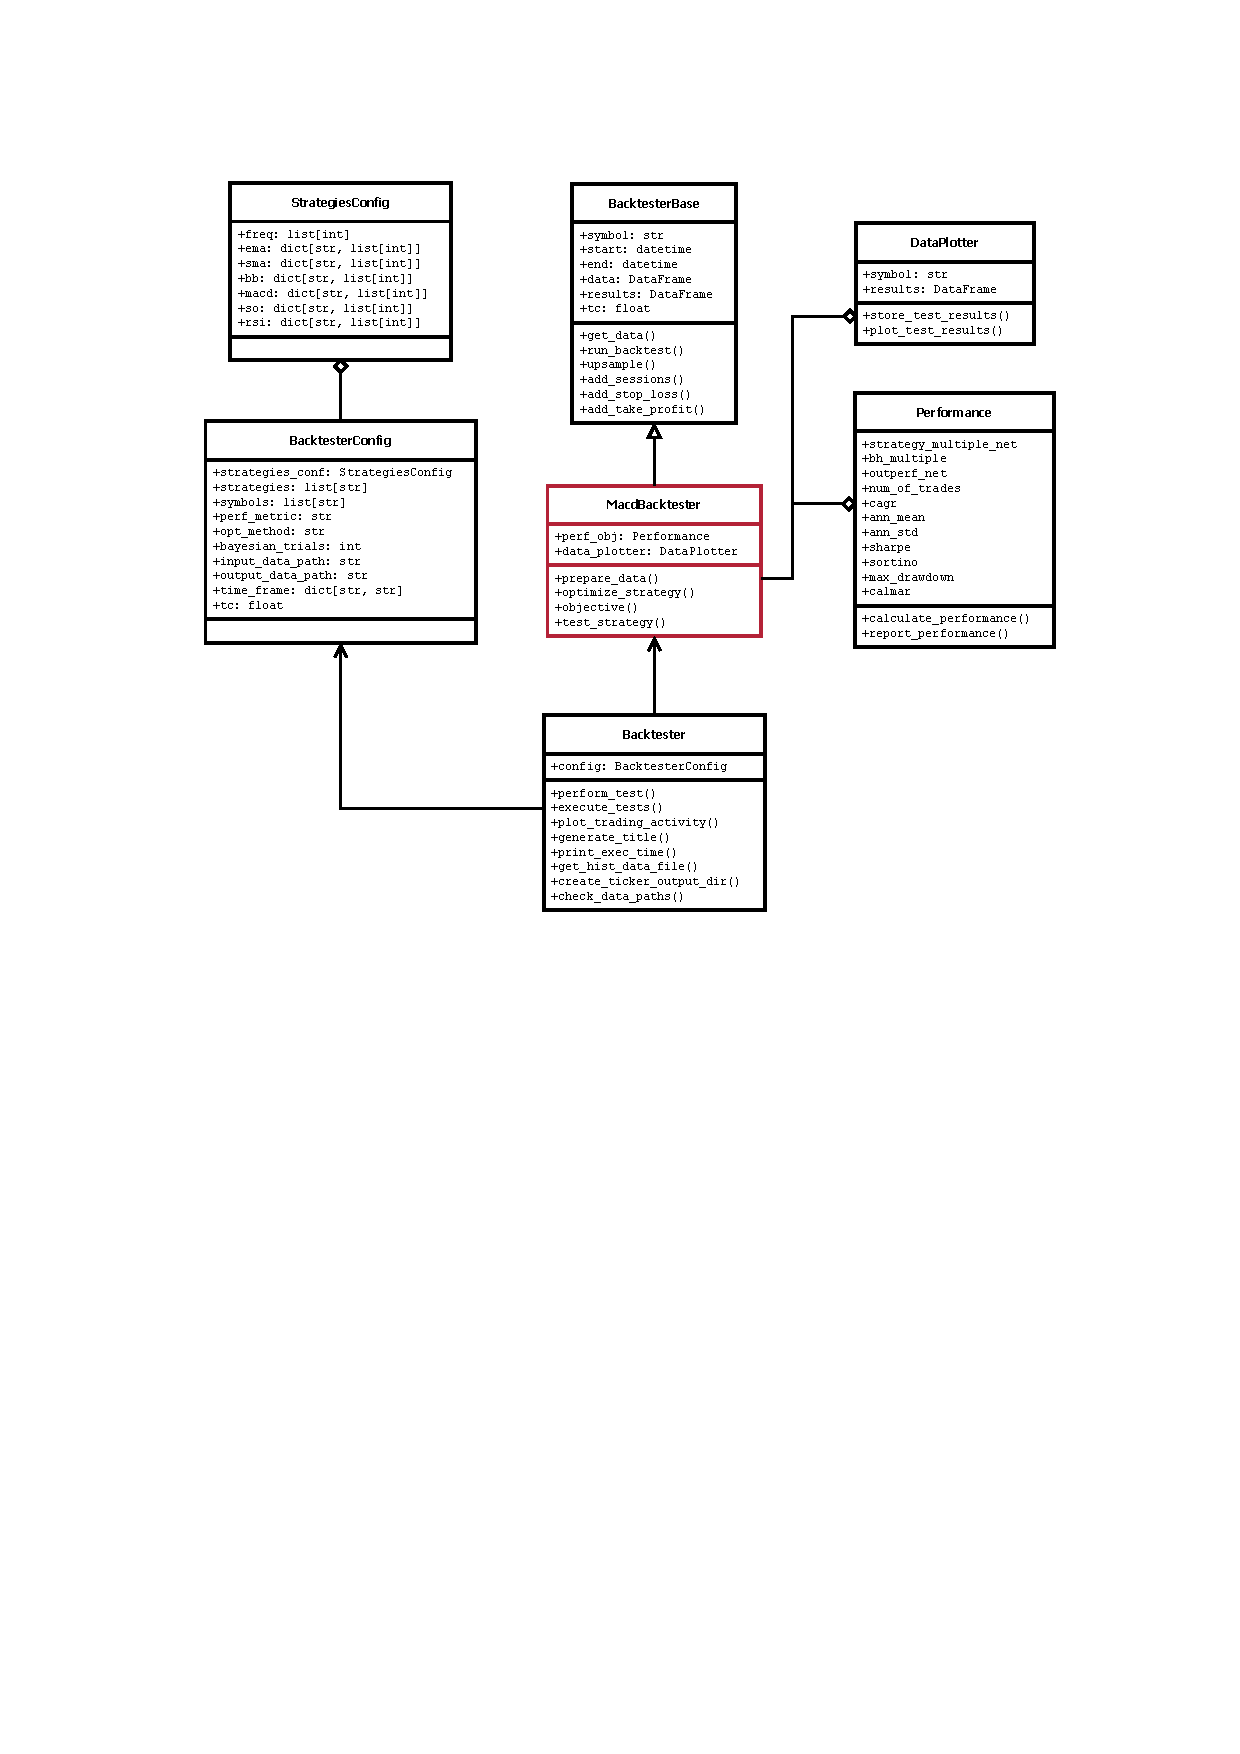
\includegraphics[page=1, trim=30mm 135mm 0 25mm, width=1.1\textwidth, clip]{./uml/backtester_uml.pdf}
\caption{Technical indicator based backtesting architecture.}
\label{fig:tech_indicator_arch}
\end{figure}

\noindent
Technical indicators are mathematical calculations based on historical price, volume, or open interest information that aim to predict future price movements.
Commonly used in technical analysis, these indicators provide insight into the market's direction, strength, momentum, and volatility.

The cornerstone of this framework lies in its automated, vectorized backtesting, which furnishes a remarkably efficient backtesting utility.
The framework incorporates two distinct backtesting variations: one for machine learning-based models and another for technical indicator-based models.
A notable feature of the framework is its extensibility; new testing algorithms can be seamlessly incorporated and configured.
For integration, each new algorithm should inherit from the \texttt{BacktesterBase} class, located in the \texttt{backtester\_base.py} module.
Furthermore, they must implement the methods: \texttt{prepare\_data}, \texttt{optimize\_strategy}, \texttt{objective()}, and \texttt{test\_strategy()}.

Figure \ref{fig:tech_indicator_arch} delves into the architecture of the technical indicator-based backtesting component within the framework.
Notably, the UML class (delineated in red) titled \texttt{MacdBacktester} is a descendant of the \texttt{BacktesterBase} class.
This base class equips all models with essential methods such as \texttt{get\_data}, \texttt{run\_backtest}, \texttt{add\_stop\_loss}, and \texttt{add\_take\_profit}, to name a few.
Additional classes, namely \texttt{DataPlotter} and \texttt{Performance}, are harnessed to compute and graphically represent performance metrics for each test.

A pivotal aspect of this framework is the adaptability of each algorithm's parameters.
Users have the flexibility to configure the parameter spaces via the JSON file named \texttt{backtesterconfig}.
This configuration is subsequently ingested and validated through \texttt{pydantic}.
For optimization, users can employ either the grid search method or the Bayesian method.
While grid search explores all possible combinations in the parameter space, the Bayesian approach uses probability distributions to improve the search.
Given the configuration of parameter spaces for each algorithm, numerous combinations---potentially tens of thousands---can be tested for each symbol.
The performance results for all these combinations are consolidated into a single CSV file, facilitating subsequent analysis.

Consider the snapshot below, extracted from a more intricate configuration, as a case in point:
\begin{verbatim}
{
    "opt_method": "bayesian",
    "bayesian_trials": 1500,
    "time_frame": {
      "start_date": "",
      "end_date": "2022-12-31 23:59:00"
    },
    "symbols": ["XRPUSDT", "LTCUSDT", "TRXUSDT"],
    "strategies_config":
    {
      "freq" : [5, 125, 5],

      "ema": {
          "ema_s": [6, 60, 4],
          "ema_l": [10, 200, 5]
      }
    }
}
\end{verbatim}



Furthermore, individual backtesting results for each symbol and strategy can be visualized, as depicted in fig.~\ref{fig:backtest_results}.
This figure showcases the performance results of the optimized strategy juxtaposed against the buy-and-hold strategy.
As an illustrative example, the EMA strategy for LTCUSDT is spotlighted. All pertinent parameters are illustrated above the primary plot.
Testing was executed on historical data spanning from 2021-01-01 to 2021-12-31.
The secondary plot, detailing close prices, accentuates the drastic price fluctuations during this period.
 Impressively, the algorithm managed to surpass the buy-and-hold strategy, achieving an outperformance of 0.953 (which can be construed as a 95\% enhancement).

\begin{table}[ht!]
    \centering
    \begin{tabular}{l}
        \texttt{LTCUSDT | EMA : (plot\_all = True , freq = 125 , ema\_s\_val = 50 , ema\_l\_val = 200 )} \\
        \texttt{Strategy Multiple = 2.065 , Buy/Hold Multiple = 1.09 ,} \\
        \texttt{Net Out-/Under Perf = 0.953 , Num Trades = 14} \\
    \end{tabular}
\end{table}


\begin{figure}[ht!]
\centering
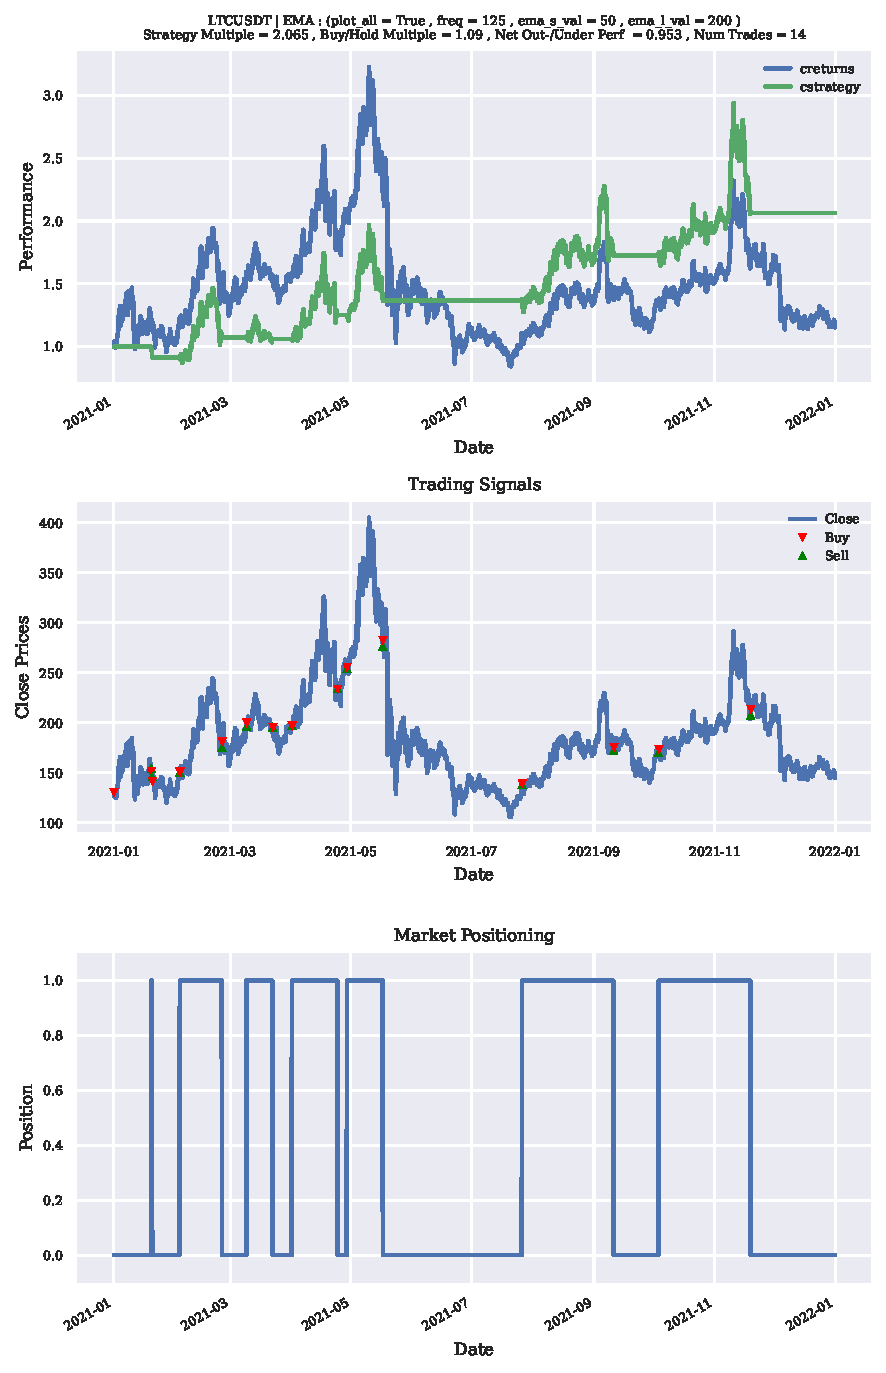
\includegraphics[page=1, trim=0mm 0mm 0 0mm, width=1\textwidth, clip]{./uml/backtesting_results.pdf}
\caption{Results of Backtesting of MACD Stragegy of XRPUSDT.}
\label{fig:backtest_results}
\end{figure}

